\section{Finite-Difference Method for Unsteady Open Channel Flow}
%%%%%%%%%%%%%%%%%%%%%%%%%%%
Solving the St. Venant Equations is accomplished by mapping the physical system and the
set of partial differential equations into an algebraic structure that a computer can manipulate.
Finite-difference, finite-element, finite-volume, and marker-in-cell are the typical methods.
The simplest form of solution that is conditionally stable and reasonably straightforward to
program is called the Lax-Diffusion scheme.

This scheme is reasonably accurate and useful for practical problems as well as to learn what
goes on under the hood of a professional tool like HEC-RAS.
\subsection{Governing Difference Equations -- Lax Scheme}
The finite-difference analysis converts the two PDEs into an algebraic update structure and
maps boundary conditions onto a computational domain.
The two PDEs are continuity and momentum; they are coupled in the same sense as they were in the water-hammer part of pipeline flow -- the resulting difference scheme will look quite similar.
\subsubsection{Continunity}
The continuity equation for a computational cell (reach) is 
\begin{equation}
\frac{\partial y}{\partial t} = -\frac{A}{B}\frac{\partial V}{\partial x}-V\frac{\partial y}{\partial x}
\end{equation}

$A$ is the depth-area function (a function of x and y). 
$B$ is the depth-topwidth function (a function of x and y). 
The Lax scheme uses spatial averaging to represent the $A$, $B$, and $V$ terms that appear as coefficients on the partial derivatives on the right-hand side of the equation. 
The time derivative is accomplished with a conventional forward-in-time first order finite difference model, and the spatial derivatives are conventional first-order centered differences.

\subsubsection{Momentum}
The momentum equation is
\begin{equation}
\frac{\partial V}{\partial t} = g(S_0-S_f)-V\frac{\partial V}{\partial x}-g\frac{\partial y}{\partial x}
\end{equation}
and also uses spatial averages for the coefficients on the spatial derivatives in the right hand side of the equation as well as spatial averages for the friction and topographic slopes. 
Friction slope can be recovered using any resistance model, Chezy-Manning's is typical.

\subsection{Mapping from the Physical to Computational Domain}
The next important step is to map the physical world to the computer world.

\begin{figure}[h!] %  figure placement: here, top, bottom, or page
   \centering
   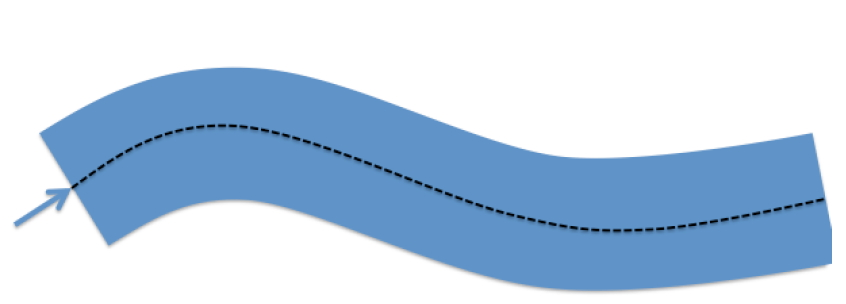
\includegraphics[width=3.6in]{stream-schematic.jpg} 
   \caption{Plan view of a stream.  Flow in figure is from left to right}
   \label{fig:stream-schematic}
\end{figure}

Figure \ref{fig:stream-schematic} is a schematic of a stream that is to be modeled. 
The stream has some width, depth, and path. 
The dashed line in the figure is the thalweg and is the pathline of the stream. 
Distances in the computational model are along this path. 
The conventional orientation is ``looking downstream." 
So when the cross sections are stationed the distances in a cross section are usually referenced as distanced from the left bank, looking downstream.

Figure \ref{fig:stream-section-schematic} is a schematic that depicts the relationship of left-bank, cross section, elevations, and such -- all referenced to the concept of ``looking downstream."

\begin{figure}[h!] %  figure placement: here, top, bottom, or page
   \centering
   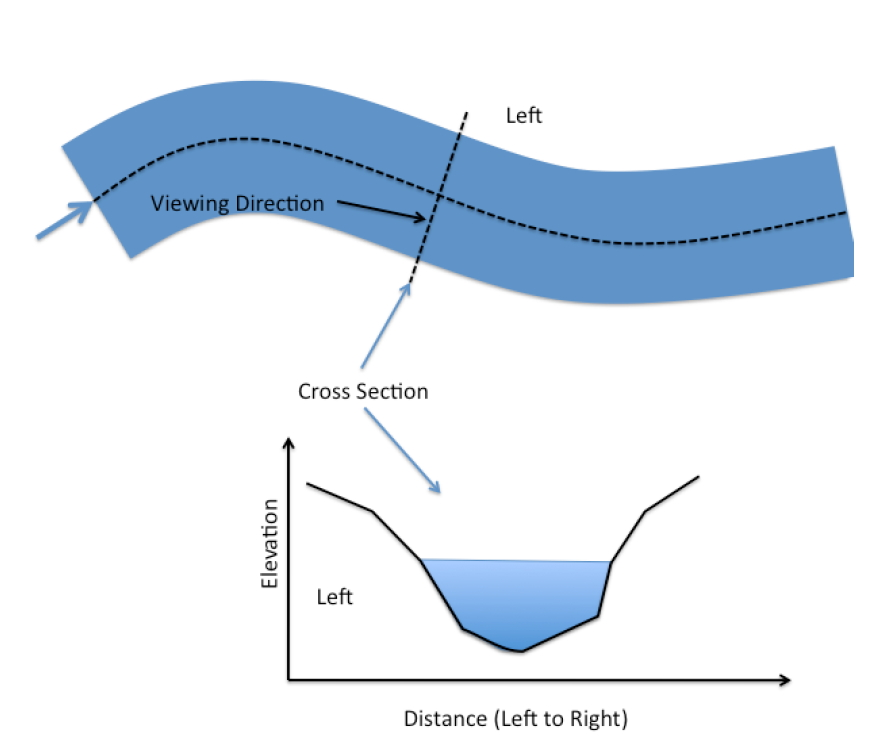
\includegraphics[width=3.6in]{stream-section-schematic.jpg} 
   \caption{Schematic of relationship of cross-section, elevation, and left bank}
   \label{fig:stream-section-schematic}
\end{figure}
\newpage

Figure \ref{fig:stream-discritize} is a schematic of the next step of mapping into the computational domain. 

\begin{figure}[h!] %  figure placement: here, top, bottom, or page
   \centering
   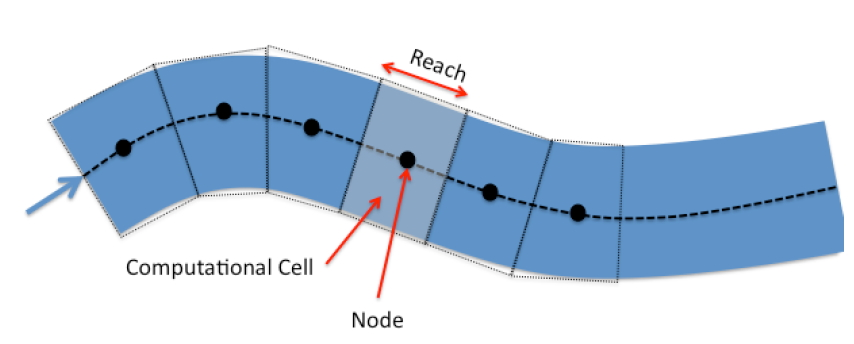
\includegraphics[width=4in]{stream-discritize.jpg} 
   \caption{Schematic of physical interpretation of a reach, cell, and node}
   \label{fig:stream-discritize}
\end{figure}

In the figure the stream is divided into cells called reaches (or cells, depends on context and author).
The centroid of the reach is canned the node, and most of the arithmetic is written with the
understanding that all properties of the reach are somehow ``averaged" and these averages
are assigned to these nodes. 
Adjacent nodes are connected (in the computer) by links.
The continuity and momentum equations collectively describe the node average behavior (such
as depth) and link behavior (such as momentum flux).

Figure \ref{fig:stream-node-scheme} is a schematic of three adjacent nodes that is used to develop the difference equations.

\begin{figure}[h!] %  figure placement: here, top, bottom, or page
   \centering
   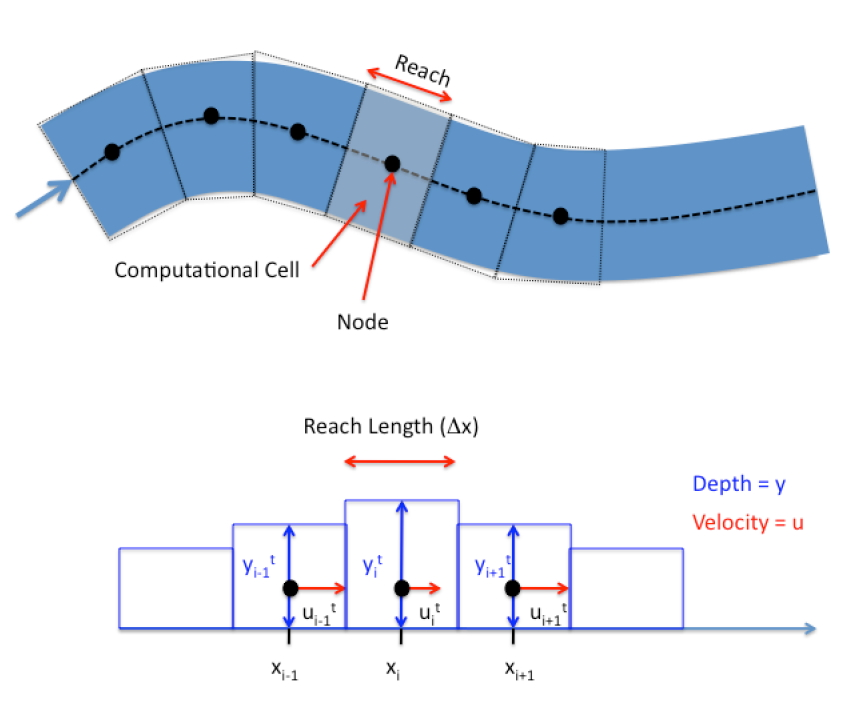
\includegraphics[width=4.25in]{stream-node-scheme.jpg} 
   \caption{Schematic of three adjacent nodes, with average depth and section velocity depicted \textbf{at the node}.
   Different schemes map these quantities to different places in the cell -- often velocities are at cell interfaces}
   \label{fig:stream-node-scheme}
\end{figure}

In the figure both the velocities and depths are mapped to the node (Lax-Diffusion scheme), but other schemes map the velocities to the interfaces. 
Again this decision affects the differencing scheme; the differencing scheme
chooses the location. 
A kind of chicken and egg situation. 

At this point the mapping has abstracted considerably from the physical world and the computer world loses sense of
sinuosity. 
In this development, we will assume the reach lengths are all the same value, the velocities are all parallel to the local thalweg and perpendicular to the cross sections, and the depth is measured from the channel bottom.
The differencing scheme then replaces the continuity and momentum PDEs with update
equations to map the water surface position and mean section velocity at the nodes to different moments in time. 
The updating is called time-stepping.

\subsection{Building the Difference Equations}
The partial derivatives are replaced with difference quotients that approximate their behavior.  
The mapping in some sense influences the resulting difference scheme.  

\subsubsection{Time Differences}
The naive time difference is 
\begin{equation}
\frac{\partial y}{\partial t}~\approx~\frac{y_i^{t+\Delta t}-y_i^t}{\Delta t}
\end{equation}
Lax replaced the known time-level term with its spatial average from adjacent cells.
For the depth;
\begin{equation}
\frac{\partial y}{\partial t}~\approx~\frac{y_i^{t+\Delta t}-\frac{1}{2}(y_{i-1}^t+y_{i+1}^t}{\Delta t}
\end{equation}
Similarly for mean section velocity
\begin{equation}
\frac{\partial V}{\partial t}~\approx~\frac{V_i^{t+\Delta t}-\frac{1}{2}(V_{i-1}^t+V_{i+1}^t}{\Delta t}
\end{equation}

\subsubsection{Space Differences}
Lax used centered differences for the spatial derivatives
\begin{equation}
\frac{\partial y}{\partial x}~\approx~\frac{y_{i+1}^{t}-y_{i-1}^t}{2\Delta x}
\end{equation}

\begin{equation}
\frac{\partial V}{\partial x}~\approx~\frac{V_{i+1}^{t}-V_{i-1}^t}{2\Delta x}
\end{equation}
Lax also used spatial averages for the depth-area and slope functions
\begin{equation}
\frac{1}{2}(\frac{A}{B}\vert_{i-1}^t + \frac{A}{B}\vert_{i+1}^t)
\end{equation}
\begin{equation}
\frac{1}{2}(S_{f,i-1}^t + S_{f,i+1}^t)
\end{equation}

These difference formulations are substituted into continunity and momentum and then rearranged to isolate the terms at the $t+\Delta t$ time level.

\subsubsection{Continunity}
Starting with the PDE,
\begin{equation}
\frac{\partial y}{\partial t} = -\frac{A}{B}\frac{\partial V}{\partial x}-V\frac{\partial y}{\partial x}
\end{equation}
first replace the time derivative
\begin{equation}
\frac{y_i^{t+\Delta t}-\frac{1}{2}(y_{i-1}^t+y_{i+1}^t}{\Delta t} = -\frac{A}{B}\frac{\partial V}{\partial x}-V\frac{\partial y}{\partial x}
\end{equation}
then replace the space derivatives
\begin{equation}
\frac{y_i^{t+\Delta t}-\frac{1}{2}(y_{i-1}^t+y_{i+1}^t}{\Delta t} = -\frac{A}{B}\frac{V_{i+1}^{t}-V_{i-1}^t}{2\Delta x}-V\frac{y_{i+1}^{t}-y_{i-1}^t}{2\Delta x}
\end{equation}
then the spatial averages for the remaining terms.
\begin{equation}
\begin{matrix}
\frac{y_i^{t+\Delta t}-\frac{1}{2}(y_{i-1}^t+y_{i+1}^t)}{\Delta t} = -\frac{1}{2}(\frac{A}{B}\vert_{i-1}^t + \frac{A}{B}\vert_{i+1}^t)\frac{V_{i+1}^{t}-V_{i-1}^t}{2\Delta x}-\frac{1}{2}(V_{f,i-1}^t + V_{f,i+1}^t)\frac{y_{i+1}^{t}-y_{i-1}^t}{2\Delta x}\\
~\\
 \end{matrix}
\end{equation}
Next multiply by $\Delta t$
\begin{equation}
\begin{matrix}
y_i^{t+\Delta t}-\frac{1}{2}(y_{i-1}^t+y_{i+1}^t) = -\Delta t\frac{1}{2}(\frac{A}{B}\vert_{i-1}^t + \frac{A}{B}\vert_{i+1}^t)\frac{V_{i+1}^{t}-V_{i-1}^t}{2\Delta x}-\Delta t \frac{1}{2}(V_{f,i-1}^t + V_{f,i+1}^t)\frac{y_{i+1}^{t}-y_{i-1}^t}{2\Delta x}\\
~\\
 \end{matrix}
\end{equation}
Move the time level $t$ term to the right hand side
\begin{equation}
\begin{matrix}
y_i^{t+\Delta t} = \frac{1}{2}(y_{i-1}^t+y_{i+1}^t) -\Delta t\frac{1}{2}(\frac{A}{B}\vert_{i-1}^t + \frac{A}{B}\vert_{i+1}^t)\frac{V_{i+1}^{t}-V_{i-1}^t}{2\Delta x}-\Delta t \frac{1}{2}(V_{f,i-1}^t + V_{f,i+1}^t)\frac{y_{i+1}^{t}-y_{i-1}^t}{2\Delta x}\\
~\\
 \end{matrix}
\end{equation}
Rename the constant  $\frac{\Delta t}{2 \Delta x} = r$ and simplify
\begin{equation}
\begin{matrix}
y_i^{t+\Delta t} = \frac{1}{2}(y_{i-1}^t+y_{i+1}^t) -\frac{r}{2}(\frac{A}{B}\vert_{i-1}^t + \frac{A}{B}\vert_{i+1}^t)(V_{i+1}^{t}-V_{i-1}^t)-\frac{r}{2}(V_{f,i-1}^t + V_{f,i+1}^t)(y_{i+1}^{t}-y_{i-1}^t) \\
~\\
 \end{matrix}
 \label{eqn:lax-continunity}
\end{equation}

\subsubsection{Momentum}
Again, starting with the PDE, make the time substitution
\begin{equation}
\frac{V_i^{t+\Delta t}-\frac{1}{2}(V_{i-1}^t+V_{i+1}^t)}{\Delta t} = g(S_0-S_f)-V\frac{\partial V}{\partial x}-g\frac{\partial y}{\partial x}
\end{equation}
next the space derivatives
\begin{equation}
\begin{matrix}
\frac{V_i^{t+\Delta t}-\frac{1}{2}(V_{i-1}^t+V_{i+1}^t)}{\Delta t} = g(S_0-S_f)-V\frac{V_{i+1}^{t}-V_{i-1}^t}{2\Delta x}-g\frac{y_{i+1}^{t}-y_{i-1}^t}{2\Delta x}\\
~\\
\end{matrix}
\end{equation}
then the spatial averages\footnote{If the channel slope is changing, then this would be subjected to a spatial averaging scheme too!}
\begin{equation}
\begin{matrix}
\frac{V_i^{t+\Delta t}-\frac{1}{2}(V_{i-1}^t+V_{i+1}^t)}{\Delta t} = 
g(S_0-\frac{1}{2}(S_{f,i-1}^t + S_{f,i+1}^t))
-\frac{1}{2}(V_{i-1}^t+V_{i+1}^t) \frac{V_{i+1}^{t}-V_{i-1}^t}{2\Delta x}
-g\frac{y_{i+1}^{t}-y_{i-1}^t}{2\Delta x}\\
~\\
\end{matrix}
\end{equation}
Multiply by $\Delta t$
\begin{equation}
\begin{matrix}
V_i^{t+\Delta t}-\frac{1}{2}(V_{i-1}^t+V_{i+1}^t)= 
\Delta t  g(S_0-\frac{1}{2}(S_{f,i-1}^t + S_{f,i+1}^t))
-\Delta t  \frac{1}{2}(V_{i-1}^t+V_{i+1}^t) \frac{V_{i+1}^{t}-V_{i-1}^t}{2\Delta x}
-\Delta t  g\frac{y_{i+1}^{t}-y_{i-1}^t}{2\Delta x}\\
~\\
\end{matrix}
\end{equation}
Rename the constant  $\frac{\Delta t}{2 \Delta x} = r$ and isolate the $t + \Delta t$ term
\begin{equation}
\begin{matrix}
V_i^{t+\Delta t}=\frac{1}{2}(V_{i-1}^t+V_{i+1}^t) +
\Delta t  g(S_0-\frac{1}{2}(S_{f,i-1}^t + S_{f,i+1}^t))
- \frac{r}{2}(V_{i-1}^t+V_{i+1}^t) (V_{i+1}^{t}-V_{i-1}^t)
-rg(y_{i+1}^{t}-y_{i-1}^t)\\
~\\
\end{matrix}
\label{eqn:lax-momentum}
\end{equation}

The pair of update equations, Equation \ref{eqn:lax-continunity} and \ref{eqn:lax-momentum} are the interior point update equations.

Figure \ref{fig:space-time-map} depicts the updating information transfer. 
At each cell the three known values of a variable ($y$ or $V$) are projected to the next time line as depicted in the figure.
Boundary conditions are the next challenge.
These are usually handled using characteristic equations (unless the boundaries are really simple).

\begin{figure}[h!] %  figure placement: here, top, bottom, or page
   \centering
   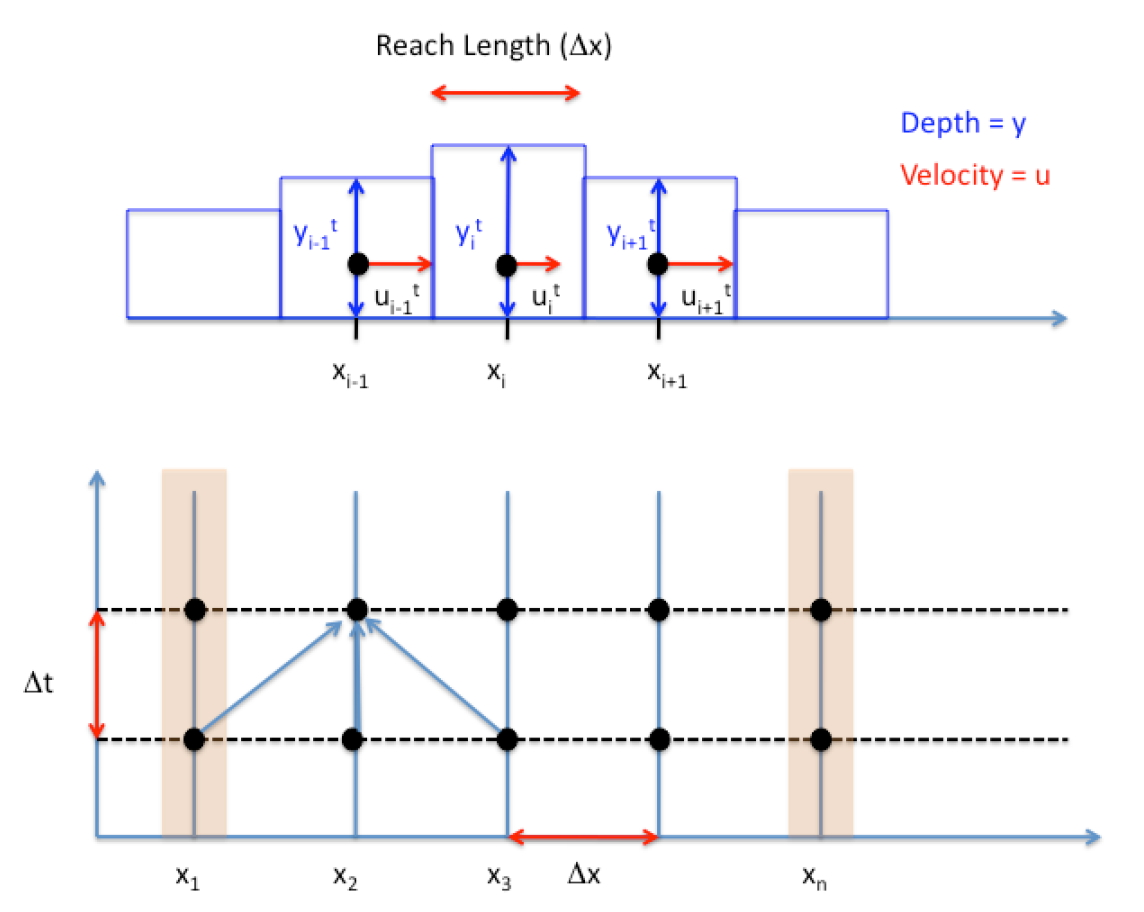
\includegraphics[width=4.25in]{space-time-map.jpg} 
   \caption{Relation of the linked reaches to solution of the equations in the XT-plane. Explicit updating (as used herein) uses the three values at the known time level to project (update) the unknown value at the next time level. 
Boundary behavior is an independent calculation, dependent on the evolution of the interior solution}
   \label{fig:space-time-map}
\end{figure}

\subsubsection{Example 1 -- Steady flow in a rectangular channel}
The backwater curve situation for a rectangular channel with discharge over a weir is repeated.  
The channel width is 5 meters, bottom slope $0.001$, Manning's $n=0.02$ and discharge $Q=55.4 \frac{m^3}{sec}$.
We will start with the flow depth artificially large and observe that the transient solver will eventually produce an equilibrium solution that is the same as the steady-flow solver.  
Generally such a simulation is a good idea to test a new algorithm -- it should be stable enough to convereg to and maintain a steady solution.

A script that implements these concepts is listed on the next several pages.
The script is comprised of several parts, and for the sake of taking advantage of the ability of \textbf{R} to read and operate on files, the script will have several ``libraries'' that read by a main control program.
The main program controls the overall solution process, while the library functions can be built and tested in advance.

First are prototype functions for the hydraulic components associated with the channel geometry, shown on listing \ref{lst:hydraulic-functions}.

\begin{lstlisting}[caption=R code demonstrating prototype hydraulic functions, label=lst:hydraulic-functions]
# hydraulic functions -- save in file named <lax-diffusion-hydraulics-lib.R>
# depth == flow depth          
# bottom == bottom width of trapezoidal channel
# side == side slope (same value both sides) of trapezoidal channel
# computed values:
# bt == computed topwidth :: ar == flow area, used in fd update :: wp == wetted perimeter, used in fd update
bt <- function(depth,bottom,side){   # depth-topwidth function
 topwidth <- (bottom + 2.0*side*depth);
 return(topwidth);
} # tested 12MAR2015 TGC
ar <- function(depth,bottom,side){   # depth area function
 area <- (depth*(bottom+side*depth));
 return(area)
} # tested 12MAR2015 TGC
# depth perimeter
wp <- function(depth,bottom,side){   
 perimeter <- (bottom+2.0*depth*sqrt(1.0+side*side));
 return(perimeter)
} # tested 12MAR2015 TGC
\end{lstlisting}

The next set of functions are prototype functions for reporting the output -- it will be cleaner to build the output functions separate from the control program, and send the necessary vectors when we want to actually print results.
Listing \ref{lst:display-functions} is a listing of such functions (albeit specific to the particular code).

\begin{lstlisting}[caption=R code demonstrating prototype display (printing) functions, label=lst:display-functions]
# display functions -- save in a file named <lax-diffusion-display-lib.R>
###### Message Functions #####################
writenow <- function(t,dt,y,v,b0,s) { # printing functions
message("__________")
message("Time = ",t," seconds.","Time step length = ",dt," seconds ")
aa <- ar(y,b0,s);
qq <- aa*v
brb <- bt(y,b0,s)
ww <- wp(y,b0,s)
message("--in write now----")
print(cbind(y,qq,v,qq,brb,ww,zz))
message("-----------------")
return()  #observe a NULL return, this function messages to the output device, so there is nothing to return.
}
###### Plotting Functions #####################
plotnow<-function(t,x,y,v){
 mainlabel=c("Flow Depth at time = ",t," seconds")
	plot(x,y,main=mainlabel,xlab="distance (m)",ylab="depth (m)",xlim=c(0,30000),ylim=c(0,15),type="l",lwd=3,col="blue")
	lines(x,v,lwd=3,col="red",type="l")
return()  #observe a NULL return, this function plots to the graphics device, so there is nothing to return.
	}
\end{lstlisting}



\begin{lstlisting}[caption=R code demonstrating prototype finite-difference formulation/function, label=lst:finite-difference-functions]
###### Finite Difference Functions ############
finitedifference<-function(){
r <- 0.5*dt/dx;
###### LEFT BOUNDARY ##########
## MODIFY TO A REFLECTION BOUNDARY ##
## THEN SUPPLY DISCHARGE TO THE FIRST CELL AND USE CONTINUNITY TO FIND DEPTH ##
##  qq is the interpolated hydrograph flow value
#debug message("left boundary ",qq$y)
#debug message("left boundary ",y[1])
#######################################################
vp[1] <<- qq$y/ar(y[1],b0,s);
ab <- ar(y[2],b0,s);
bb <- bt(y[2],b0,s);
cb <- sqrt(g*bb/ab);
rb <- ab/wp(y[2],b0,s);
sfb <- (mn2*v[2]*v[2])/(rb^(1.333));
#debug print(cbind(ab,bb,cb,rb,sfb));
cn <- v[2] -cb*y[2]+ g*(s0-sfb)*dt;
yp[1] <<- (vp[1] - cn )/cb;
######################################################
### gives y,v at location 1 time level k+1
#debug message("--left bndry ----")
#debug print(cbind(y,yp,v,vp,sfb,cn,rb));
######## RIGHT BOUNDARY ##############
## MODIFY TO A FREE OUTFALL
## USE A WEIR EQUATION BASED ON SOME REFERENCE DEPTH
vp[nn]<<- (y[n]-yd)*sqrt(9.8*y[n]);
## USE CHARACTERISTIC LINE TO FIND ASSOCIATED DEPTH
 aa <- ar(y[n],b0,s);
 ba <- bt(y[n],b0,s);
 ca <- sqrt(g*ba/aa);
 ra <- aa/wp(y[n],b0,s);
 sfa <- (mn2*v[n]*v[n])/(ra^(4.0/3.0));
 cp <- v[n] + ca*y[n]+g*(s0-sfa)*dt;
 yp[nn] <<- (cp - vp[nn])/ca;
#  ## fixed stage
# yp[nn] <<- yd ;
# aa <- ar(y[n],b0,s);
# ba <- bt(y[n],b0,s);
# ca <- sqrt(g*ba/aa);
# ra <- aa/wp(y[n],b0,s);
# sfa <- (mn2*v[n]*v[n])/(ra^(4.0/3.0));
# cp <- v[n] + ca*y[n]+g*(s0-sfa)*dt;
# vp[nn] <<- (cp - ca*yp[nn]); # check sign
#   message("--right bndry ----")
# print(cbind(y,yp,v,vp));

# reflection boundary, find depth along a characteristic
# vp[nn] <<-0 ;
# aa <- ar(y[n],b0,s);
# ba <- bt(y[n],b0,s);
# ca <- sqrt(g*ba/aa);
# ra <- aa/wp(y[n],b0,s);
# sfa <- (mn2*v[n]*v[n])/(ra^(4.0/3.0));
# cp <- v[n] + ca*y[n]+g*(s0-sfa)*dt;
# yp[nn] <<- (cp - vp[nn])/ca;
##print(cbind(y,yp,v,vp));
######## INTERIOR NODES AND REACHES ###############
# loop through the interior nodes
for (i in 2:n){ # begin interior node loop scope
aa <- ar(y[i-1],b0,s);
ba <- bt(y[i-1],b0,s);
pa <- wp(y[i-1],b0,s);
ra <- aa/pa;
sfa <- (mn2*v[i-1]*v[i-1])/(ra^(4.0/3.0));
ab <- ar(y[i+1],b0,s);
bb <- bt(y[i+1],b0,s);
pb <- wp(y[i+1],b0,s);
rb <- ab/pb;
sfb <- (mn2*v[i+1]*v[i+1])/(rb^(4.0/3.0));
# need averages of sf, hydraulic depth
dm <- 0.5*(aa/ba + ab/bb);
sfm <- 0.5*(sfa+sfb);
vm <- 0.5*(v[i-1]+v[i+1]);
ym <- 0.5*(y[i-1]+y[i+1]);
# update momentum
# note the double <<, this structure forces the
# value to be global and accessible
# to other functions when the script is run
vp[i] <<- vm -r*g*(y[i+1] - y[i-1]) -r*vm*(v[i+1] - v[i-1]) + g*dt*(s0-sfm);
# update depth
yp[i] <<- ym - r*dm*(v[i+1] - v[i-1]) -r*vm*(y[i+1] - y[i-1]);
} # end of interior node loop scope
} # end of function scope
\end{lstlisting}

\begin{lstlisting}[caption=R code demonstrating prototype updating function, label=lst:update-functions]

###### Solution Update Function ###########
update<-function(y,yp,v,vp){
y <<- yp;
v <<- vp;
return()
}
### NEED ADAPTIVE TIME STEPPING FOR THE FLOOD WAVE 
###### Adaptive Time Step Functions ###########
## here is where we do adaptive time stepping
bestdt<-function(y,v){
  bestdt <- dt # start with current time step
  for (i in 1:nn){
    a <- ar(y[i],b0,s);
    b <- bt(y[i],b0,s);
    c <- sqrt(g*a/b);
    dtn <- dx/abs((v[i])+c)
    # now test
    if(dtn <= bestdt){bestdt <- dtn}
  } # end loop scope
  dt <<- bestdt
} #end bestdt function
###### Solution Update Function ###########
update<-function(y,yp,v,vp){
  y <<- yp;
  v <<- vp;
  return()
}
\end{lstlisting}

[Present the problem, and important features -- then to solution listed below.  Uses the library]



\subsubsection{Example 2 -- Routing a storm hydrograph}
The initial depth in a horizontal channel of rectangular cross section is 1 meter.
The channel is 29 kilometers long and ends with a non-reflection boundary condition.
The initial discharge in the channel is 0 cubic meters per second.
The upstream input hydrograph is shown in Figure \ref{fig:upstreamHydro}.
The manning friction factor is $n=1/40$.  
Simulate the water surface elevation over time in the channel.

\begin{figure}[h!] %  figure placement: here, top, bottom, or page
   \centering
   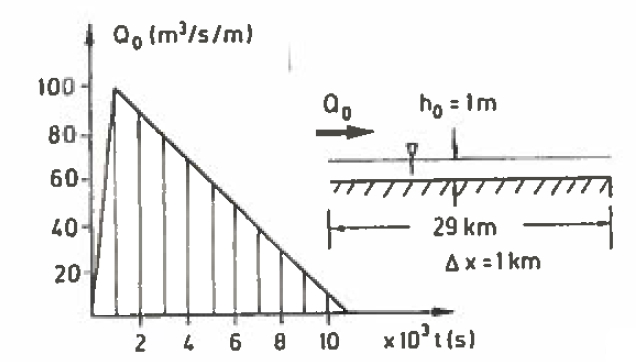
\includegraphics[width=4.25in]{upstreamHydro.jpg} 
   \caption{Upstream hydrograph for example}
   \label{fig:upstreamHydro}
\end{figure}

\subsubsection{Example 3 -- Sudden gate closing in an aqueduct channel}
To illustrate a script to implement these concepts consider the example problem:\\
Flow in a 1000-m long trapezoidal channel with a bottom width of 20-m, side slope of 2H:1V, longitudinal slope $S_0$=0.0001, and Manning's resistance n=0.013. 
Initial discharge in the channel is 110 m3/s and initial flow depth is 3.069 m.
Simulate the flow and depth at every 100-m station when a downstream gate is closed at t=0. 
Produce a graph of depth and velocity versus location for t=0, 60, 360 seconds.

\subsubsection{Example 4 -- Long waves in a tidal-influenced channel}


\subsection{Appendix}
Listing \ref{lst:Lax Scheme Implementation} is a listing of a Lax Scheme as a single file.

\begin{lstlisting}[caption=R code for Lax Scheme, label=lst:Lax Scheme Implementation]

# main program for st. venant
rm(list=ls())
setwd("~/Dropbox/CE5361-2015-1/Project2/Project2-Problem2")
# clear workspace and set directory
source('~/Dropbox/CE5361-2015-1/Project2/Project2-Problem2/Project2.2.Lib.R')

###### Problem Constants #######
# these are constants that define the problem
# change for different problems
# a good habit is to assign constants to names so the
# program is readable by people in a few years
g <-9.81 # gravitational acceleration, obviously SI units
n <- 29 # number of reaches
#q0 <- 110 # initial discharge
q0 <- 11 # initial discharge
#yd <- 3.069 # initial flow depth in the model
yd <- 1.000 # initial flow depth in the model
#yu <- 3.069 # upstream constant depth
yu <- 1.1 # upstream constant depth
# mn <- 0.013 # Manning's n
mn <- 0.02 # Manning's n
# b0 <- 20 # bottom width
b0 <- 5 # bottom width
## modify for problem 1 s0 <- 0.0001 # longitudinal slope (along direction of flow)
s0 <- 0.0000001 # longitudinal slope (along direction of flow)
#s  <- 2.0 # side slope (passed to calls to hydraulic variables)
s  <- 0.0 # side slope (passed to calls to hydraulic variables)
l  <- 30000.0 # total length (the lenght of computational domain)
tmax <- 640000 # total simulation time in seconds
iprt <- 8 # print every iprt time steps
nn <- n+1 # how many nodes, will jack with boundaries later
mn2 <- mn*mn # Manning's n squared, will appear a lot.
a <- ar(yd,b0,s) # flow area at beginning of time
v0 <- q0/a # initial velocity
######## Here we build vectors ###############
y <- numeric(nn) # create nn elements of vector y
yp <- numeric(nn) # updates go in this vector, same length as y
v <- numeric(nn) # create nn elements of vecotr v
vp <-numeric(nn) # updates go in this vector, same length and v
ytmp <-numeric(nn)
vtmp <-numeric(nn)
y <- rep(yd,nn) # populate y with nn things, each thing has value yd
v <- rep(v0,nn) # populate v with nn things, each thing has value v0
b <- bt(yd,b0,s) # topwidth at beginning
c <- sqrt(g*a/b) # celerity at initial conditions
###
hydrograph <- numeric(1)
dummy<- read.csv(file="hydrograph.csv",header=F)
elapsedtime <- dummy$V1; # forst column of hydrograph is time
hydrograph <- dummy$V2; # second column of hydrograph is flow
print(cbind(c))
dx <- l/n # delta x, length of a reach
xx <- dx*seq(1:nn)-1000  # Spatial locations of nodes, used for plotting
zz <- 30 - s0*xx # bottom channel elevation
dt <- dx/(v0 + c) # the time step that satisfies the courant condtions
kmax <- round(tmax/dt)  # set maximum number of time steps
print(cbind(dx,dt))



### Run the simulation                  ###
k <- 0 # time counter
t <- 0.0 # elapsed time
pdf("junk2.2.plot.pdf") # graphics device for plots -- plotnow() sends data to plot
writenow(t,dt,y,v,b0,s)  # Write initial conditions
plotnow(t,xx,y,v)
####### BEGIN TIME STEPPING ########
message("kmax =", kmax)
for (itime in 1:kmax){
## put in the hydrograph here -- use approx function to interpolate
## we are after the second value qq$y in the approx function
qq <<- approx(elapsedtime,hydrograph,t)
print (qq$x);
print (qq$y);
#debug print(qq$y) 
#############  NEED ADAPTIVE TIME STEPPING FOR THE HYDROGRAPH ROUTING #############
bestdt(y,v);
############# THIS IS A HACK TO GET STABILITY #################
# halve the time step 
dt <- dt/16 
finitedifference(); # Finite difference a single time step
#update(ytmp,yp,vtmp,vp); # Update vectors
#update(y,yp,v,vp); # Update vectors
#bestdt(yp,vp)
message("dt now = ",dt);
#finitedifference(); # Finite difference a single time step
ytmp <- (yp+ytmp)/2;
vtmp <- (vp+vtmp)/2;
update(y,yp,v,vp); # Update vectors
message(" dt is ",dt);
t <- t+dt; # Increment simulation time
k <- k+1; # Increment loop counter
if (k%%iprt == 0){writenow(t,dt,y,v,b0,s)}; # Write current conditions every iprt time steps
if (k%%iprt == 0){plotnow(t,xx[seq(1,nn,1)],(y[seq(1,nn,1)]),(v[seq(1,nn,1)]))}; # Plot current solution
# reset the time step
############ UNHACK TO KEEP ADAPTIVE TIME STEPPING WORKING ###########
dt <- 16*dt
}
dev.off() # disconnect the pdf file.
\end{lstlisting}
%%